\documentclass[10pt,a4paper]{article}
\usepackage[margin=1.9cm,top=1.7cm,bottom=1.7cm]{geometry}
\usepackage[T1]{fontenc}
\usepackage{lmodern,microtype}
\usepackage{graphicx,booktabs,amsmath,amssymb,tikz,xcolor,caption,enumitem,hyperref}
\usetikzlibrary{arrows.meta,positioning}
\captionsetup{font=small,labelfont=bf,skip=3pt}
\setlength{\parindent}{0pt}\setlength{\parskip}{3pt}
\renewcommand{\textfraction}{0.05}\renewcommand{\topfraction}{0.95}
\setlist{nosep,leftmargin=1.2em}
\hypersetup{colorlinks,linkcolor=blue!50!black,citecolor=blue!50!black,urlcolor=blue!50!black}
\usepackage{titlesec}
\titleformat{\section}{\large\bfseries}{\thesection}{0.5em}{}
\titlespacing*{\section}{0pt}{7pt}{2pt}

\begin{document}
\begin{center}
{\Large\bfseries How fast is fast enough? Quantifying the epidemiological impact of reducing the symptom-onset-to-isolation delay}\\[3pt]
{\bfseries Team TAUS:} Oluwafemi Samson Olagbami, Humphrey Rop, Imelda Laetitia Simboro, Jonathan Boakye-Yiadom\\
{\small Advisers: Dr.\ James Azam, Andrej Jarynowski \quad|\quad All members contributed equally \quad|\quad Preliminary results, 31 October 2026\\
Code and data: GitHub repository submitted with this report (\texttt{run\_all.sh} regenerates every figure and number)}
\end{center}
\vspace{-4pt}
\begin{abstract}\noindent
\textbf{Abstract.} The 2026 Bundibugyo virus disease (BVD) outbreak in the Democratic Republic of the Congo (DRC) has passed 10,000 confirmed cases, and confirmed incidence has stayed near 70 per day since August. We asked how many cases would be prevented, and how much sooner the outbreak would end, if the mean delay from symptom onset to isolation fell from 7 to 5 or 3 days, with isolation that is 50\%, 80\% or 100\% effective. We built a deterministic SEIQR model with an isolation rate equal to one over the delay, calibrated it to the observed flat incidence (effective reproduction number $R_e\approx1.0$), and propagated uncertainty through 1,000 parameter draws and a stochastic check. Over 12 months, a 5-day delay averts 52--86\% of cases and a 3-day delay 77--95\% (95\% uncertainty intervals 38--99\%), depending on isolation effectiveness. At 80\% effectiveness, a 3-day delay brings $R_e$ to 0.74 and ends the outbreak in about 9 months, versus about 24 months at 5 days; at 7 days it does not end.
\end{abstract}

\section{Introduction}
In May 2026 the DRC declared an outbreak of Bundibugyo virus disease, now the second-largest Ebola-disease outbreak on record, with a case-fatality ratio of about 48\% among confirmed cases \cite{zomahoun,kabasele}. By 28 October 2026, 10,274 cases and 4,992 deaths had been confirmed in the DRC \cite{cdc}. Response teams face a concrete operational question: every day between first symptoms and isolation is a day in which a patient can infect household members, carers and health workers. The study brief puts the first-month delay between symptom onset and sampling at 7.4 days, and the late-August surveillance review found contact tracing below all targets, only 15--20\% of new cases already known as contacts, and 59\% of confirmed deaths occurring outside treatment units \cite{kabasele}. Community engagement, decentralised testing and transit centres all aim to shorten this delay, but the benefit of doing so is not directly observable by field teams.

Earlier Ebola work showed that isolation lowers the reproduction number, and that the combined speed of diagnosis and the effectiveness of isolation determine whether control succeeds \cite{chowell}. Scenario models for this outbreak have varied the \emph{fraction} isolated with a fixed 2-day delay \cite{mooring}, but we are not aware of a public estimate of the benefit of shortening the delay itself when isolation is imperfect. \textbf{Research question:} among symptomatic infectious people in this outbreak, how would reducing the mean onset-to-isolation delay from 7 to 5 and 3 days change cumulative cases and outbreak duration under worst-, base- and best-case isolation effectiveness (50\%, 80\%, 100\%)?

\section{Methods}
\textbf{Model.} We use a deterministic compartmental model (Figure~\ref{fig:model}; equations in the Appendix). People are susceptible (S), exposed but not yet infectious (E), infectious and not yet isolated (I), isolated but still infectious (Q), or recovered/removed (R). Infectious people are isolated at rate $\tau=1/\text{delay}$, so the mean time to isolation is the delay being studied; they leave I otherwise by recovery or death at rate $\gamma$. Isolation is imperfect: isolated people transmit at a fraction $1-\epsilon$ of the rate of non-isolated people, where $\epsilon=$ 0.5, 0.8 or 1 is the \emph{isolation effectiveness}. A deterministic model was chosen for transparent scenario comparison; a stochastic binomial-chain version checks that the conclusions survive chance events.

\begin{figure}[h]
\centering
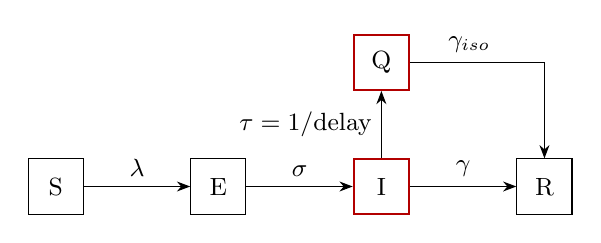
\begin{tikzpicture}[node distance=1.35cm,>=Stealth,box/.style={draw,minimum size=0.7cm,inner sep=2pt},every node/.style={font=\small}]
\node[box](S){S}; \node[box,right=of S](E){E}; \node[box,right=of E,draw=red!70!black,thick](I){I};
\node[box,right=of I](R){R}; \node[box,above=0.85cm of I,draw=red!70!black,thick](Q){Q};
\draw[->](S)--node[above]{$\lambda$}(E); \draw[->](E)--node[above]{$\sigma$}(I);
\draw[->](I)--node[above]{$\gamma$}(R); \draw[->](I)--node[left]{$\tau=1/\text{delay}$}(Q);
\draw[->](Q)-|node[above,pos=0.22]{$\gamma_{iso}$}(R);
\end{tikzpicture}
\caption{Model structure. The studied intervention is the flow I$\to$Q (rate $\tau$). Force of infection $\lambda=\beta[I+(1-\epsilon)Q]/N$, where $\epsilon$ is the isolation effectiveness.}\label{fig:model}
\end{figure}

\textbf{Data and calibration.} We compiled cumulative confirmed DRC cases from published reports (\texttt{data/}, 8 dated counts with sources; early counts from \cite{akem}). Confirmed incidence in the four intervals between 2 June (363) and 28 October (10,274) was 64, 76, 68 and 70 cases per day, i.e.\ essentially flat. A log-linear fit gave a growth rate $r=0.0009$ per day (95\% CI $-0.0044$ to $0.0061$; only 2 degrees of freedom). The model starts on 28 October with 70 new symptomatic cases per day and the corresponding E, I, Q distribution. Transmission $\beta$ is calibrated so that the \emph{7-day baseline} reproduces this growth rate, separately for each $\epsilon$; scenarios then change only $\tau$. ``Cases'' therefore means confirmed symptomatic cases; under-ascertainment is not modelled.

\begin{table}[h]
\centering\small
\caption{Parameters. Triangular distributions (minimum, mode, maximum) were sampled independently.}\label{tab:par}
\begin{tabular}{@{}llp{7.4cm}@{}}\toprule
Parameter & Value & Source \\\midrule
Mean latent period $1/\sigma$ & 4.0, 6.3, 10.1 d & Akilimali et al.\ model input \cite{akilimali}; upper bound from \cite{chowell}\\
Mean infectious period $1/\gamma=1/\gamma_{iso}$ & 5, 7, 10 d & \cite{akilimali}; 6.5 d in \cite{chowell}\\
Current growth rate $r$ & 0.0009 (SE 0.0012), Student-$t_2$ & Fitted to \texttt{data/}\\
Onset-to-isolation delay & 7, 5, 3 d (scenarios) & Study brief; 4.6 d onset-to-sample and 8.6 d onset-to-result in \cite{akilimali}\\
Isolation effectiveness $\epsilon$ & 0.5, 0.8, 1.0 (scenarios) & Worst/base/best case\\
Population $N$; horizon & $10^7$; 365 d & Depletion negligible\\\bottomrule
\end{tabular}
\end{table}

\textbf{Scenarios and outcomes.} Nine scenarios cross three delays (7, 5, 3 days) with three effectiveness levels. Primary outcomes are cumulative symptomatic cases over 12 months and outbreak duration, defined as the first day on which fewer than one person remains exposed or infectious. Secondary outcomes are the effective reproduction number $R_e$ (infections per case at the start) and peak incidence. Cases averted are the paired difference from the 7-day run with the same parameter draw and the same $\epsilon$. \textbf{Uncertainty:} 1,000 joint draws of latent period, infectious period and growth rate; results are medians with 95\% uncertainty intervals (UI). We also ran 500 stochastic replicates per scenario, a global sensitivity analysis (partial rank correlation over latent period, infectious period, growth rate, $\epsilon\in[0.5,1]$ and delay $\in[3,7]$ d), and changed the baseline delay to 4.6 and 8.6 days.

\section{Results}
\textbf{Baseline.} With a 7-day delay the model reproduces the flat incidence: $R_e\approx1.01$ (95\% UI 0.94--1.09) and about 28,800 confirmed symptomatic cases over the next 12 months (UI 13,000--111,000; the width reflects how little the four data intervals constrain $r$). The same figure results at every $\epsilon$ because $\beta$ is recalibrated.

\textbf{Shorter delays.} Every faster delay turns flat incidence into decline (Figure~\ref{fig:traj}; Table~\ref{tab:res}), so peak incidence equals the starting level of about 70 per day and the time to peak is zero in all intervention scenarios. Moving from 7 to 5 days averts 52\% of cases if isolation is 50\% effective (UI 38--64\%), 75\% at 80\% (61--87\%) and 86\% at 100\% (73--94\%). Moving to 3 days averts 77\% (62--88\%), 90\% (80--97\%) and 95\% (88--99\%) (Figure~\ref{fig:av}a). In absolute terms, at 80\% effectiveness a 3-day delay averts about 26,000 cases (UI 10,000--107,000). Absolute averted-case intervals are wide because they scale with the uncertain baseline growth; percentages are more stable.

\begin{figure}[t]
\centering\includegraphics[width=\textwidth]{../figures/fig2_trajectories.pdf}
\caption{Daily new symptomatic cases (median and 95\% UI band, log scale) for the three delays at each isolation effectiveness.}\label{fig:traj}
\end{figure}

\begin{table}[t]
\centering\small
\caption{Scenario results: median (95\% UI) over 1,000 draws. Duration in months from 28 October 2026; ``no end'' = the outbreak persisted beyond 5 years in 96\% of draws. $^\dagger$Only 52\% of draws ended within 5 years; duration shown is among those.}\label{tab:res}
\input{../results/table_scenarios.tex}
\end{table}

\textbf{Effectiveness of isolation matters, but speed matters more.} At 80\% effectiveness, a 3-day delay brings $R_e$ to 0.74 (0.70--0.79) and ends the outbreak in a median of 9 months (7--13), compared with 24 months (16--45) at 5 days; at 100\% effectiveness these become 5 and 13 months. At 50\% effectiveness, $R_e$ falls below 1 for 94\% of draws at 5 days but the outbreak lasts about 4 years if it ends at all, whereas a 3-day delay ends it in about 23 months (15--40). In the global sensitivity analysis (Figure~\ref{fig:av}b) the delay had the strongest influence on 12-month cases (partial rank correlation 0.94), followed by isolation effectiveness ($-0.79$), baseline growth (0.68) and latent period (0.34); the infectious period mattered little (0.09).

\begin{figure}[t]
\centering\includegraphics[width=\textwidth]{../figures/fig3_averted_sensitivity.pdf}
\caption{(a) Percentage of 12-month cases averted relative to a 7-day delay (median, 95\% UI). (b) Global sensitivity of 12-month cases.}\label{fig:av}
\end{figure}

\textbf{Robustness.} The stochastic runs agree with the deterministic ones: baseline 29,200 cases (UI 13,000--89,000), 7,600 (4,900--15,800) for 5 days and 3,030 (2,220--4,320) for 3 days at 80\% effectiveness. In stochastic runs, the outbreak went extinct within 5 years in 98--100\% of runs at 3 days (any $\epsilon$) and 99--100\% at 5 days with $\epsilon\ge0.8$, but in only 9--17\% at 7 days. If the true current delay were already 4.6 days \cite{akilimali}, a 5-day target would raise rather than lower cases, but shortening to 3 days would still avert 81\% of cases at 80\% effectiveness; if it were 8.6 days, 5 and 3 days would avert 83\% and 92\%.

\section{Discussion}
\textbf{Decision relevance.} Under the assumption that today's response holds incidence level at about 70 confirmed cases per day, shortening the onset-to-isolation delay is the difference between a plateau and a controlled decline. Even if isolation protects only half as well as intended, a 3-day delay lowers $R_e$ below 1 and averts roughly three quarters of the next year's cases; a 5-day delay also brings $R_e$ below 1 but only marginally when isolation is 50\% effective ($R_e=0.95$), leaving a multi-year tail. This supports investment in whatever shortens the interval: community alert networks, decentralised sampling, rapid result return (the preprint \cite{akilimali} reports a mean 8.6 days from onset to test result, much longer than to sampling), and transit or isolation capacity near communities. The size of the gain depends more on delay than on any natural-history parameter, which is a reassuring property for a result that must be used before those parameters are well known. This agrees qualitatively with earlier work finding that faster diagnosis and more effective isolation jointly drive control \cite{chowell}, and extends it to a Bundibugyo setting with explicit delay scenarios.

\textbf{Limitations.} (1) The delay is modelled as an exponential waiting time, so a ``7-day'' delay isolates only half of cases before recovery or death and mixes ``fraction isolated'' with ``speed''; real delays are skewed and shorter delays also raise the fraction reached. (2) The calibration treats flat \emph{confirmed} incidence as flat transmission, but it may partly reflect laboratory throughput, and Ituri has declined while North Kivu has grown \cite{ukhsa}; the national average hides this. The growth-rate uncertainty is based on four intervals and the intervals are wide. (3) The 7-day baseline comes from the study brief; the one primary estimate we could retrieve (a preprint) gives different values for onset-to-sample and onset-to-result, which we explored but did not resolve. (4) We do not model contact tracing, health-worker infections, unsafe burials (59\% of confirmed deaths occurred outside treatment units \cite{kabasele}), or behaviour change, and we treat isolated cases as having the same infectious period; therefore absolute numbers should be read as scenario contrasts, not forecasts. (5) Cases are confirmed cases; under-ascertainment would scale absolute numbers but not percentages. (6) Parameter ranges were taken from the outbreak preprint and Chowell and Nishiura; the systematic-review database of Nash et al.\ \cite{nash} has not yet been used to refine them.

\textbf{Next steps.} Fit the model to the incidence time series with province-specific growth, model the delay as a gamma-distributed waiting time and add a fraction-reached parameter, add unsafe burial and health-care transmission pathways, replace the placeholder ranges by the Nash et al.\ database, and ask field teams for measured onset-to-isolation delays so that the baseline is not assumed.

\section*{Acknowledgements and AI use}
We thank our advisers Dr.\ James Azam and Andrej Jarynowski. Generative AI (Claude, Anthropic) was used for brainstorming, structuring the modelling workflow, explaining technical concepts, writing the analysis code, and drafting and editing this report. The team is responsible for reviewing and approving all analyses, interpretations and written content.

\begin{thebibliography}{9}\small\setlength{\itemsep}{0pt}
\bibitem{zomahoun} Zomahoun DL, Boyd MA, Honein MA, et al. Outbreak of Ebola disease caused by Bundibugyo virus. \emph{MMWR} 2026;75:293--294. doi:10.15585/mmwr.mm7522e3.
\bibitem{kabasele} Kabasele D, Meyer E, Kabore I, et al. Characteristics and monitoring of the 2026 outbreak of Ebola disease caused by Bundibugyo virus, DRC, August 2026. \emph{MMWR} 2026;75(35):554--556. doi:10.15585/mmwr.mm7535e1.
\bibitem{cdc} CDC. Ebola outbreak: current situation (data as of 28 October 2026). \url{https://www.cdc.gov/ebola/situation-summary/index.html}.
\bibitem{akilimali} Ebengo DM, Akilimali P, et al. Early epidemiological and spatial assessment of the Bundibugyo Ebola virus outbreak 2026. Epidemiological forum preprint, 12 June 2026 (not peer reviewed).
\bibitem{chowell} Chowell G, Nishiura H. Transmission dynamics and control of Ebola virus disease (EVD): a review. \emph{BMC Med} 2014;12:196. doi:10.1186/s12916-014-0196-0.
\bibitem{mooring} Mooring EQ, Koval WT, Routledge I, et al. Modeled scenario projections for the Ebola disease outbreak caused by Bundibugyo virus, 2026. \emph{MMWR} 2026;75(22):285--289.
\bibitem{nash} Nash RK, et al. Ebola virus disease mathematical models and epidemiological parameters: a systematic review. 2024. PMID 39127058.
\bibitem{ukhsa} UKHSA. Outbreaks under monitoring, weeks 36 and 39, 2026 (case counts of 7 and 27 September 2026). \url{https://www.gov.uk/government/publications/outbreaks-under-monitoring-in-2026}.
\bibitem{akem} Akem TE, Oben EC. Operational epidemiology of the early phase of the 2026 Bundibugyo virus disease outbreak in the DRC and Uganda. \emph{PLOS Glob Public Health} 2026;6(8):e0006680 (early case counts).
\end{thebibliography}

\appendix
\section*{Appendix: equations}
\small With $\lambda=\beta I/N+\beta(1-\epsilon)Q/N$:
\[
\dot S=-\lambda S,\quad \dot E=\lambda S-\sigma E,\quad \dot I=\sigma E-(\tau+\gamma)I,\quad \dot Q=\tau I-\gamma_{iso}Q,\quad \dot R=\gamma I+\gamma_{iso}Q .
\]
The effective reproduction number at the start is $R_e=\beta\left[\dfrac{1}{\tau+\gamma}+\dfrac{\tau}{\tau+\gamma}\cdot\dfrac{1-\epsilon}{\gamma_{iso}}\right]$. For each draw, $\beta$ solves $\max\,\mathrm{Re}\,\mathrm{eig}(J)=r$ at $\tau=1/7$, where $J$ is the Jacobian of $(E,I,Q)$ at $S\approx N$. Cumulative cases are $\int\sigma E\,dt$.
\end{document}
